
\section{Trapped Ion Quantum Computing} \label{sec:Trapped}
In this section we provide an introduction to the implementation details of trapped ion quantum computers (**once done possibly elaborate what exactly we cover).
The qubits in a trapped ion system are represented by individual trapped ions.
As would have been seen in a quantum mechanics class, electrons bound in atoms can occupy a certain number of possible quantum states, here 2 of these level are chosen and used as the \kz and \ko states.
Though it isn't quite as simple as that, for quantum computing we must have a way of entangling these 2 states.
To achieve that, the qubit ions are trapped in the same trap and their motion within it is coupled as a quantum system, through which entanglement is achieved.
The rest of the required features for quantum computing including state preparation, readout and quantum gates are all achieved through tuned lasers (we use the word a bit loosely, it is to mean any source of a particular type of light) and or the mentioned entanglement.
The section is largely based on the review by Bruzewicz \cite{bruzewiczTrappedionQuantumComputing2019} and for a more detailed review on the subject we recommend that.

\subsection{Ion Trapping and the Paul Trap}
% \textbf{TODO: Also, a section on cooling might be a good idea}
Ion trapping is an extensive field of expertise used for many purposes across physics and other sciences, it is an essential component of many devices and experiments that try to manipulate individual particles, molecules or so on.
For a brief sketch of what this involves, these experiments must be done in vacuum (otherwise there would be too many other atoms around) and rely on complex electric and magnetic fields to manipulate the motion of charged atoms.
For quantum computing we are interested in trapping individual ions in a stable way, and while we want to trap multiple of them (currently about 5-100 has been achieved \cite{paganoCryogenicTrappedionSystem2018}) it is important that we can tell them apart (as opposed to trapping them in bunches as is often done).

There are currently 2 dominant, suitable classes of ion traps, Penning traps which uses a combination of magnetic and electric fields, and Paul traps (also known as Quadrupole or Radio-Frequency-Quadrupole ion traps) which uses time varying electric fields.
Penning traps are able to hold larger amounts of ions and more stably (300 ion crystals have been achieved \cite{bohnetQuantumSpinDynamics2016}), however the motion of the ions themselves is much more complicated and leads to qubit manipulation being harder to perform.
Because of that Paul traps are more commonly used for quantum computers and due to the scope of this report we will focus on them.

\subsubsection{Simple Paul Trap}
Paul trap designs use time varying fields as it is not possible to confine an ion in 3D space with only static fields.
The simplest Paul trap design is composed of 4 conducting rods run in parallel to create a quadrupole electric field in the middle (\cref{fig:TIQC_RFQ_Flour} shows a demonstrative model).
Then have each of the diagonally opposite rods connected at the same voltage and have these 2 voltages be some periodic function (usually a sine or a square wave at approximately radio frequencies, hence the name) in antiphase, so that if at some time one pair is set to positive voltage, the other should be at negative voltage.
This results in a net effect of trapping a charged particle (within some range of mass to charge ratios of the ions, the setup can be used as a mass filter) along the axis of the quadrupole, why exactly this is so is well explained in (**add a source here).
Finally, for trapping along the last axis a static electric field is used, this can be achieved by for example 2 more rod segments along the quadrupole axis at either end of the whole setup, both at some positive voltage, resulting in a potential well along the axis.

\begin{figure}[H]
    \centering
    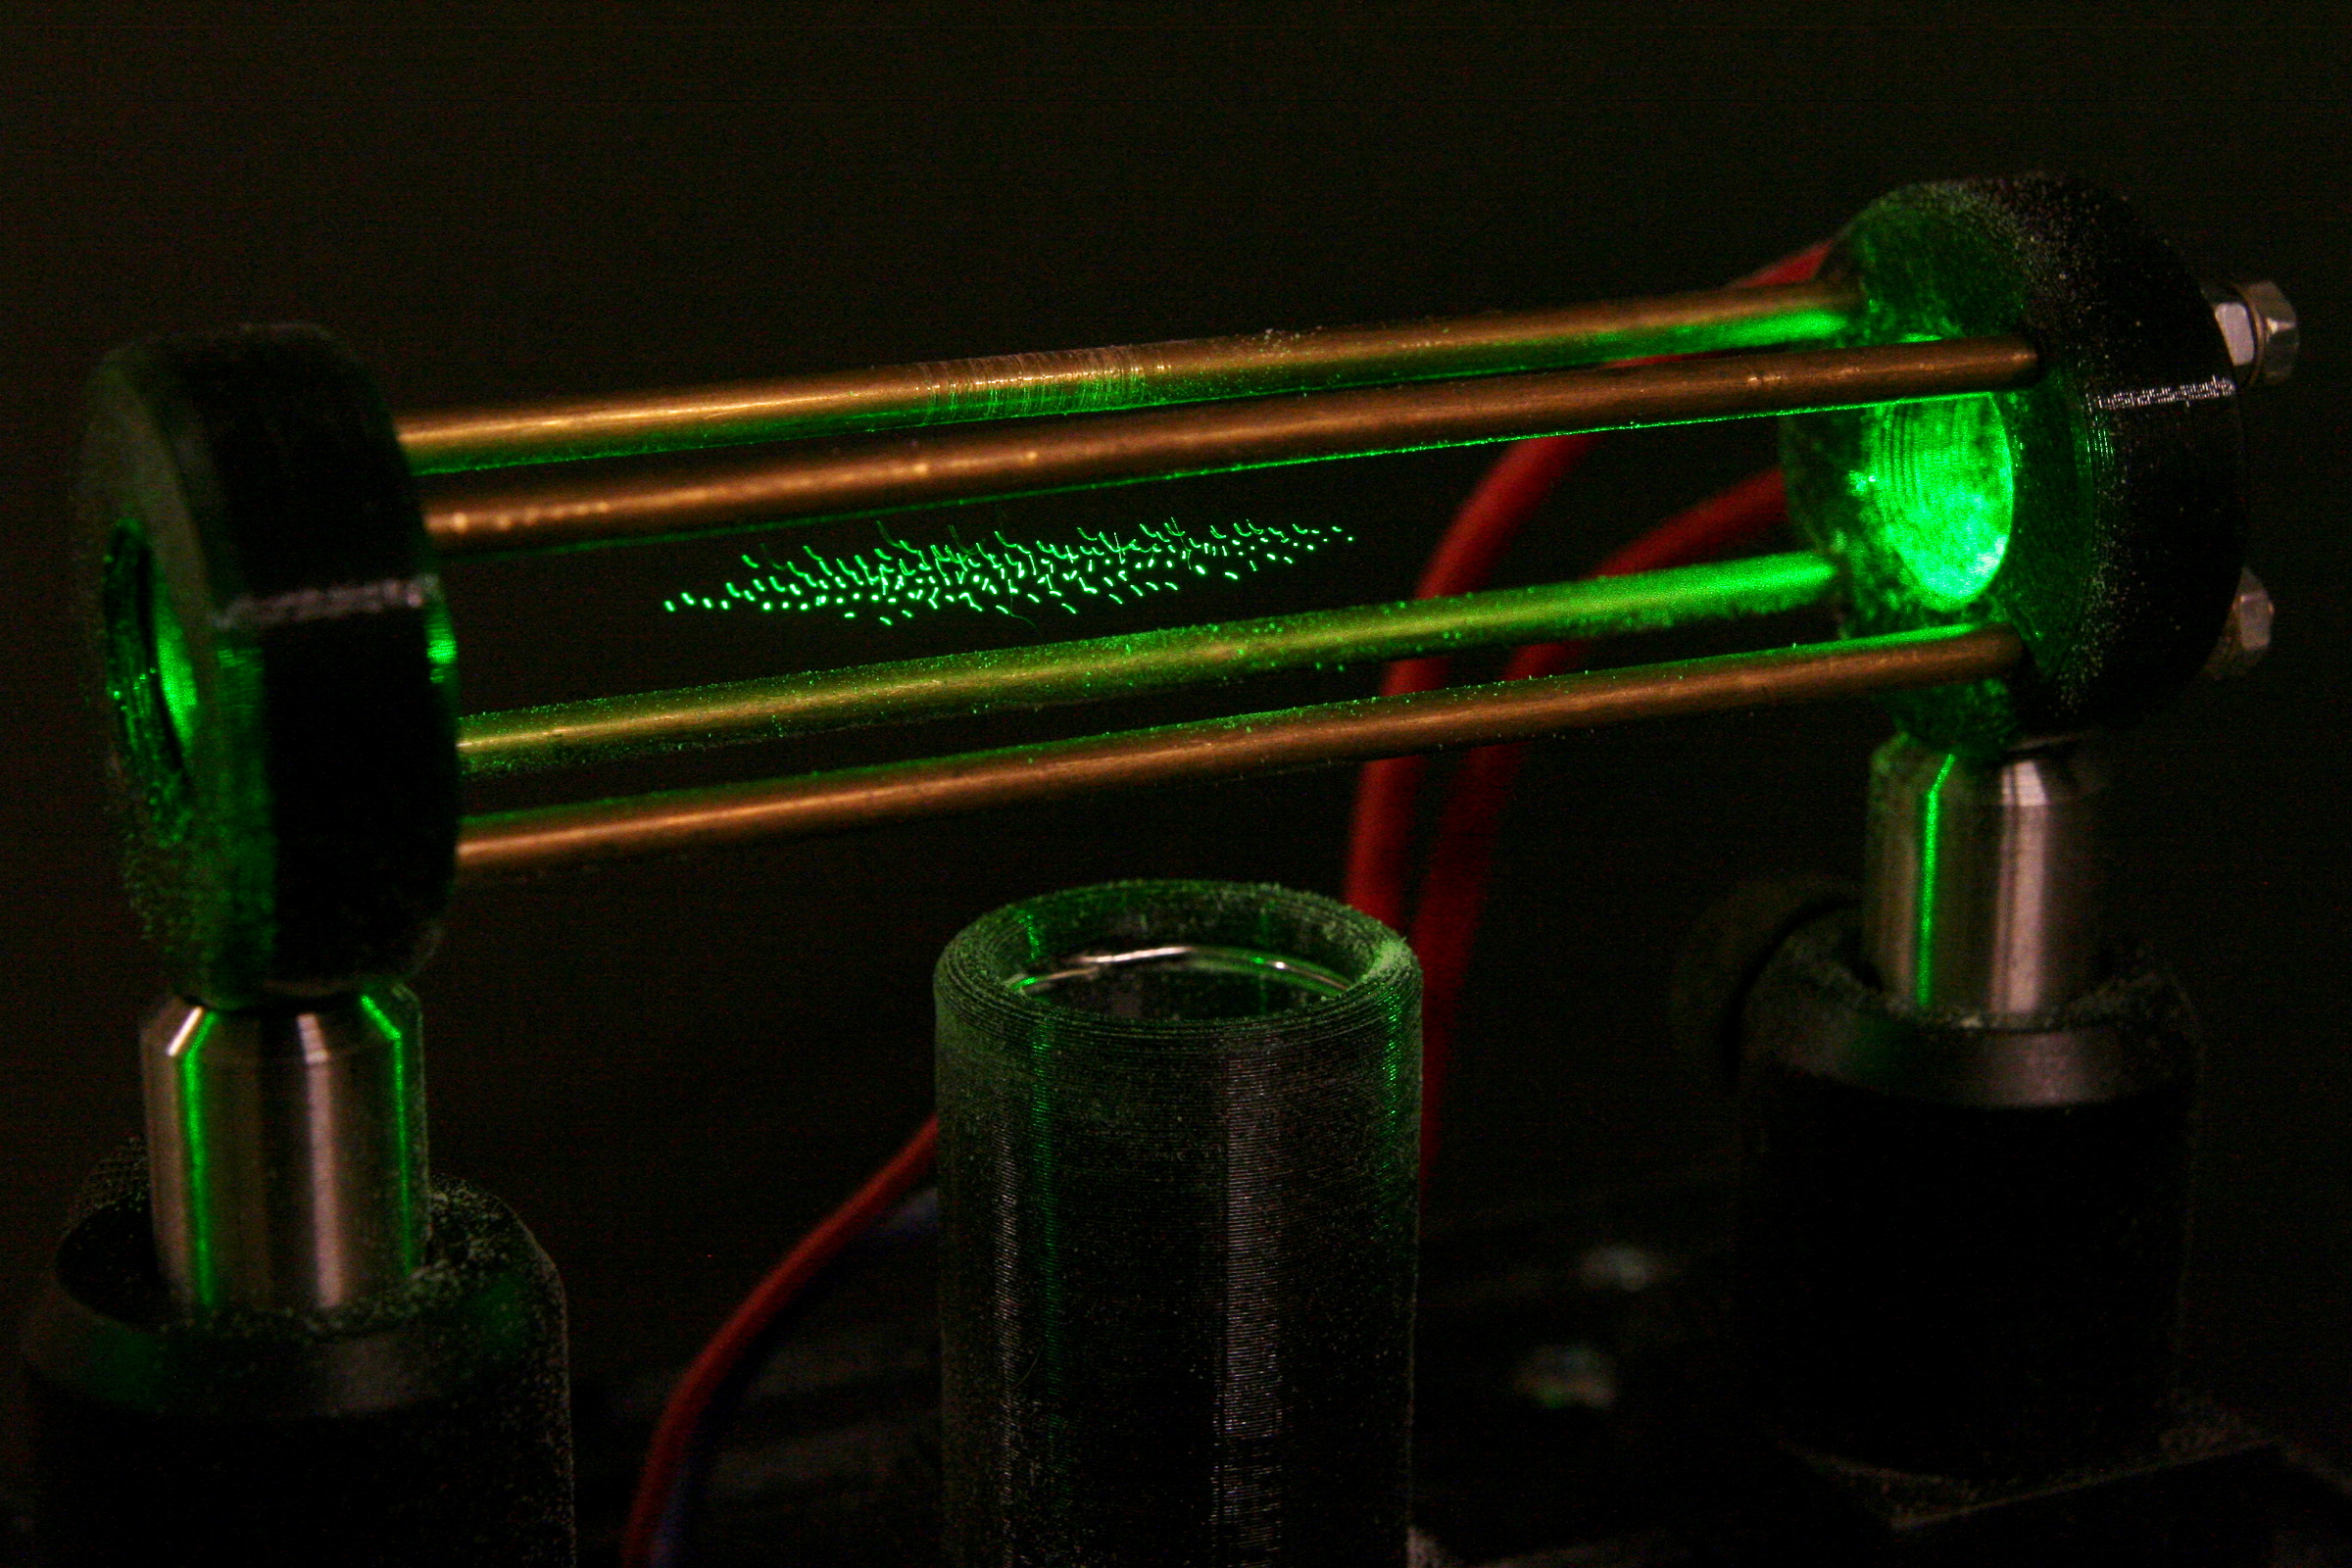
\includegraphics[width=0.9\textwidth]{images/TIQC_RFQ_Flour.jpg}
    \caption{Charged flour grains trapped in a simple Paul trap, the mentioned 4 parallel rods are visible and the electrodes creating the potential well are in the end caps.(**cite Pavelka, found on wikipedia)}\label{fig:TIQC_RFQ_Flour}
\end{figure}

\subsubsection{Notes on Other Paul Trap Designs} \label{sec:other_paultraps}
The aforementioned simple Paul trap is in fact a linear Paul trap, in this type of Paul traps the ion's motion is confined in 2 dimensions by an RF quadrupole and the last is taken care of using a linear static potential, this is the type of trap on which we will focus.
There are also point Paul traps, which utilise oscillating RF fields for trapping in all 3 dimensions, these are also used for quantum computing, however when multiple ions are trapped together (which is necessary for entanglement) their motion is significantly more complex.

However there is still a plethora of different designs being explored for further progress, most interestingly there are "surface" Paul traps.
These are usually microfabricated plates with a layout of electrodes on their surface which when driven by the correct voltages give rise to a trapping field above their surface.
These designs offer great advantages for quantum computing, as not only are they cheaper and quicker to manufacture, but can be produced with a much higher precision than manually assembled devices.
They also have the benefit of the trapped ions being much more accessible for manipulation through lasers.
Recently chips with integrated photonics have been developed too, these are surface Paul traps with optical channels running through them with openings in the surface aimed at the ion see \cref{fig:TIQC_MIT} for diagrams of one developed at MIT \cite{niffeneggerIntegratedMultiwavelengthControl2020}.
This further reduces the need for precision assembly and calibration, however complications arise with generating and maintaining entangled states if each ion is stored separately in these modules \cite{bruzewiczTrappedionQuantumComputing2019}.


\begin{figure}[H]
    \centering
    \begin{subfigure}[b]{0.45\textwidth}
        \centering
        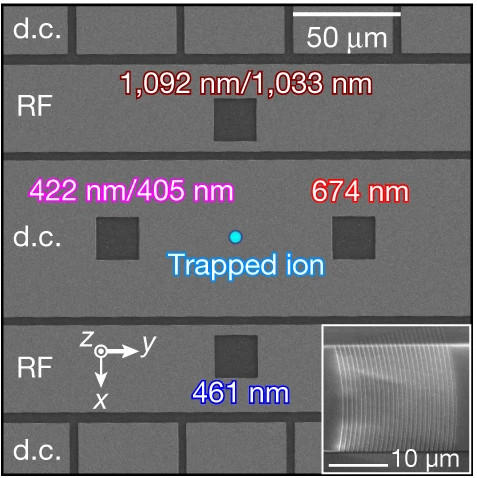
\includegraphics[width=0.9\textwidth]{images/TIQC_MIT_1.jpg}
        \subcaption{Layout of the surface Paul trap}
    \end{subfigure}
    \hfill
    \begin{subfigure}[b]{0.45\textwidth}
        \centering
        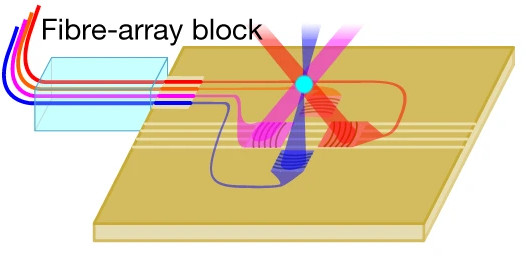
\includegraphics[width=0.9\textwidth]{images/TIQC_MIT_2.jpg}
        \subcaption{Diagram showing the photon beams}
    \end{subfigure}
    \caption{Surface Paul trap with integrated photonics for quantum computing developed at MIT in 2020.}\label{fig:TIQC_MIT}
\end{figure}

\subsection{The ions and types of qubits}
As the trapping was briefly covered, the next logical step is to focus on the ion itself.
First question is what element should be use and some of the main requirements are that it is radioactively stable, can be easily produced and singly ionized and finally that it has 2 suitable states to use as \kz and \ko from the DiVincenzo criteria.
For this, the valence electron (also the one that is "free" due to ionization) is the important part, the energy levels available to it are used as our needed states.
Typically, group 2 elements or similar (namely group 12 elements and Yb \cite{ozeriTrappedionQubitTool2011}) are used, as they are stable and have a full shell except a single valence electron -- leading to a suitable electronic structure.

For a quick summary of atomic structure, an electron is bound to the nucleus by the Coulomb interaction, if this is considered only and the quantum problem is solved, we get the gross structure, giving rise to different energy levels with different quantum numbers n.
The next step is to consider the interaction between the electrons spin and angular momentum, and also certain relativistic corrections.
This gives rise to the fine structure which are the usual orbitals described by the quantum numbers: the same n, l usually given letters s, p, d and so on, and the total spin j.
Next, there is another correction which comes from the interaction between the electron's spin and the total spin of the nucleus (if non-zero).
This gives rise to more splitting and the resulting energy levels are called the hyperfine structure.
Finally, in very vague terms, if an atom is in a magnetic field there is again more splitting, this is called the Zeeman effect.
Details on all of this can be found in \cite{woodgateELEMENTARYATOMICSTRUCTURE1970} and a diagram of the typical fine structure of the ions used for trapped ion QC along with some of the zeeman and hyperfine splittings are shown in \cref{fig:TIQC_levels}.

% some of the main requirements for a suitable isotope is that it is radioactively stable, can be produced, is singly ionizable and most importantly that the valence electron has suitable stable available quantum mechanical states to occupy, to use for \kz and \ko.
% However for many of them, there are multiple suitable electron states available for use, based on which are used the qubits would be classified as Zeeman, Hyperfine, Optical or Fine-structure.
% To summarize what these are, in either case we start with the typical electron orbitals around an atom

This gives rise to a plethora of options for the 2 levels and depending on their choice the resulting qubit can be classified into the following categories.

% Coming back to quantum computing there are many options for our states and they can usually be classified as one of following types.

\begin{figure}[H]
    \centering
    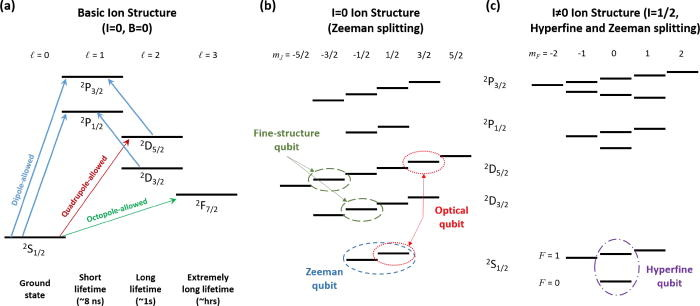
\includegraphics[width=0.9\textwidth]{images/TIQC_levels.jpeg}
    \caption{Fine structure and Zeeman and hyperfine splittings of typical atoms used for quantum computing. Some of the possible choices for the sates are also shown.}\label{fig:TIQC_levels}
\end{figure}

\paragraph{Zeeman qubits}
Zeeman qubits are qubits where the 2 states are in the same hyperfine and fine structure orbital, but result from the Zeeman effect.
They offer near infinite lifetimes and most operations can be done relatively simply, but their main drawback is that these states are very sensitive to magnetic field fluctuations (they arise from external magnetic fields after all).
This limits their coherence times, however coherence times of 300 ms have been achieved \cite{rusterLonglivedZeemanTrappedion2016}

\paragraph{Hyperfine qubits}
With these the 2 states are hyperfine split levels from the ground state.
Among their advantages are also a near infinite lifetime and possibly and an easier read out than Zeeman qubits along with a relative insensitivity to magnetic field fluctuations.
The main drawback to them is the more complicated structure of the energy levels, thus requiring greater precision in laser frequencies \cite{bruzewiczTrappedionQuantumComputing2019}.

\paragraph{Optical qubits}
With some ions it is also possible to use two fine structure levels (like an S and a D state) , this has the benefit of very simple level structure.
However the higher energy fine structure states are generally only metastable, of lifetimes on the order of seconds \cite{ozeriTrappedionQubitTool2011}.
Longer lifetimes can usually be achieved by making the manipulation laser's frequencies very precise.
However, as the energy gap is relatively big for these states, large wavelength light (visible to infrared, hence the name) has to be used for which it is difficult to achieve the required precision, though recent developments in laser technology might make them more suitable \cite{bruzewiczTrappedionQuantumComputing2019}.
The long wavelength of the manipulating lasers also results in less localised beams ($\lambda \sim \si{m}$) which means it is tough to address individual ions (cite oxford thesis 2).

\paragraph{Fine structure qubits}
This type of qubit uses 2 of the D levels mentioned in the last section.
The obvious downside is then their short lifetimes, however as the energy gap between these levels is much smaller, higher frequency precision can be more easily attained in the required lasers.
As a downside comes a more complicated level structure, for example the readout has to be done by first transferring one of the possible states to another one before reading out (cite something, probs brun.).


Overall there is not a clear winner and which choice is made depends on the particulars of the given company or research team, depending on their expertise and the equipment available to them.


\subsection{Qubit manipulation}
In the previous sections we have described how we achieve the necessary 2 states from the 1st DiVincenzo criteria, however we still have all the others to address.
All of these (ie state initialization and readout, a set of universal gates and long decoherence times) are achieved through different light beams interacting with the ions.
% These are quite complex and we only describe them at a fairly surface level, for more detail we recommend \cite{schaferFastGatesMixedSpecies2020} (the main source for this section) and specifically section 3.2 as an introduction to these phenomena.

Firstly, unsurprisingly the methods differ based on the particular quantum computer design.
To simplify things we will focus on designs where all the ions are trapped within the same trap.
A good image to have in mind is that of a linear Paul trap where we only take into account motion along the z axis, along which there is an approximately harmonic potential\footnotemark and the ions form essentially a 1D crystal through the Coulomb force interactions.
% Typically the reader can imagine a setup along the lines of a linear Paul trap where we only take into account motion along the z axis.
% Typically this is modeled along the lines of the linear Paul trap where we only take into account motion along the z axis.
% We trap some number of ions in an approximately harmonic potential\footnotemark and they form essentially a 1D crystal through the Coulomb force interactions.
It should be noted that the ions do not interact directly with each others electronic states while in the trap.
This is because they are simply too far from each other, for example \cite{schaferFastGatesMixedSpecies2020} quotes typical sizes of the ions wavefunctions to be $\sim 8 \si{\nano m}$ and the ions separations to be $\sim 3 \si{\micro m}$.

\footnotetext{This is simpler than many of the moderns systems like the ones mentioned in \cref{sec:other_paultraps}, however the while ion manipulation and entanglement is more complicated with these it is fairly analogous.}

At this point it really becomes necessary to look at the system quantum mechanically.
As the ions are within the same trap their motion is strongly coupled and can only be described together in one quantum system.
This essentially means we must look at the ions in the trap more as a collective motional wavefunction than a collection of individual atoms.
However at the same time each atom's electronic state is still kept separate and localised.
Thus we end up with essentially a register of n 2 state qubits with a shared motional state acting as a bus between them.
This motional state is also kept as simple as possible, the ions are cooled as close to the ground state as possible and often only the first excited motional state is used for gate operations.
% More detail on these topics can be found for example in 

\subsubsection{Simple light ion interactions}
While there are many ways to manipulate the ions and our qubits, all of these are achieved by shining coherent light beams at the ions.
These light ion interactions are quite complex and are studied for example in \cite{loudonQuantumTheoryLight2000}, here we only try to build some intuition for them without any real analysis.

As these are a quantum interactions, the key thing is to construct a Hamiltonian.
This being a complicated interaction however we often don't solve it directly, but expand it and only look at the first (possibly couple of the first) non-zero terms, the results are taken from \cite{schaferFastGatesMixedSpecies2020}.

\paragraph{Electric dipole interactions}
The electric dipole term is the dominant term (if not zero, this leads to certain selection rules governing when this transition can be used).
The analysis of the problem leads to the following quantum mechanical propagator\footnotemark, which can be viewed essentially as the matrix representation of the interaction's effect on the ion's state,
\footnotetext{In the Lamb-Dicke regime, when the ion's wavefunction is much smaller than the lights wavelength \cite{leibfriedQuantumDynamicsSingle2003}.}
\begin{equation}
    U = \begin{pmatrix}
        \cos{(\frac{\Omega_R t}{2})} & i \sin{(\frac{\Omega_R t}{2})} e^{-i \phi_l} \\
        i \sin{(\frac{\Omega_R t}{2})} e^{i \phi_l} & \cos{(\frac{\Omega_R t}{2})} \\
    \end{pmatrix}
\end{equation}
here $\Omega_R$ is the Rabi frequency which depends on the choice energy levels and the electric field amplitude of the incoming light, so it can be set.
Further $t$ is the time for which the light acts (how long the pulse was) and $\phi_l$ the phase of the laser light at the ion, so it can be manipulated by tuning the laser source position relative to the ion.
% Further $t$ is the time (the effect of the light will depend on how long it was turned on for) and $\phi_l$ the phase of the laser light at the ion, so it can be manipulated by tuning the laser source position relative to the ion.
This form of propagator then results in what is called Rabi oscillations, the state will be changing in some deterministic way periodically in time.

In summary then as $\Omega_R$ and $\phi_l$ can be almost arbitrarily chosen we can choose in what way it oscillates, and by choosing the time for which the laser is kept on we can achieve any rotation of the qubit on the Bloch sphere \cite{schaferFastGatesMixedSpecies2020}.
Electric dipole transitions are usually preferred due to their simplicity and speed, however they are rarely available for the needed gate transitions, though they are often used as a part of state preparation or other qubit manipulations.
% Electric dipole transitions are generally preferred both due to their relative simplicity and as they involve the highest energies and so allow very short wavelengths of the light (allowing for better localisation), however they are rarely available for the given states.

\paragraph{Magnetic dipole and electric quadrupole interactions}
If an electric dipole transition cannot be used, the next leading contributions are the magnetic dipole and electric quadrupole interactions \cite{schaferFastGatesMixedSpecies2020}.
While the Hamiltonian is very different, under certain conditions it results in a very similar propagator and also gives rise to Rabi oscillations and the same gate logic can be achieved as when using the electric dipole transition.
These type of transitions can be used with certain species of hyperfine qubits, however as microwave to radio frequency light is required, the level of addressability is limited \cite{bruzewiczTrappedionQuantumComputing2019}.

\paragraph{Raman interactions}
This is a more complicated process where to induce a transition between two states, we use two light beams to couple each of them to a third state.
Say we want a transition between the \kz and \ko states, we need to find a suitable state $\ket{2}$ with a higher energy than both.
Then we choose an energy offset $\Delta$ (and possibly $\delta$) and tune our two lasers to the differences between the $\ket{2}$ energy minus $\Delta$ and the energies of the \kz and \ko (possibly plus $\delta$) states, this is visualized in \cref{fig:TIQC_raman}.
The energy offset $\Delta$ is very important to suppress the possible transitions to state $\ket{2}$, once tuned the transition can be neglected.
The frequencies of light beams is usually denoted $\omega_b$ and $\omega_r$, standing for "blue" and "red" with the blue being the more energetic, this often carries through into terms like blue/red sideband transitions and similar.

\begin{figure}[H]
    \centering
    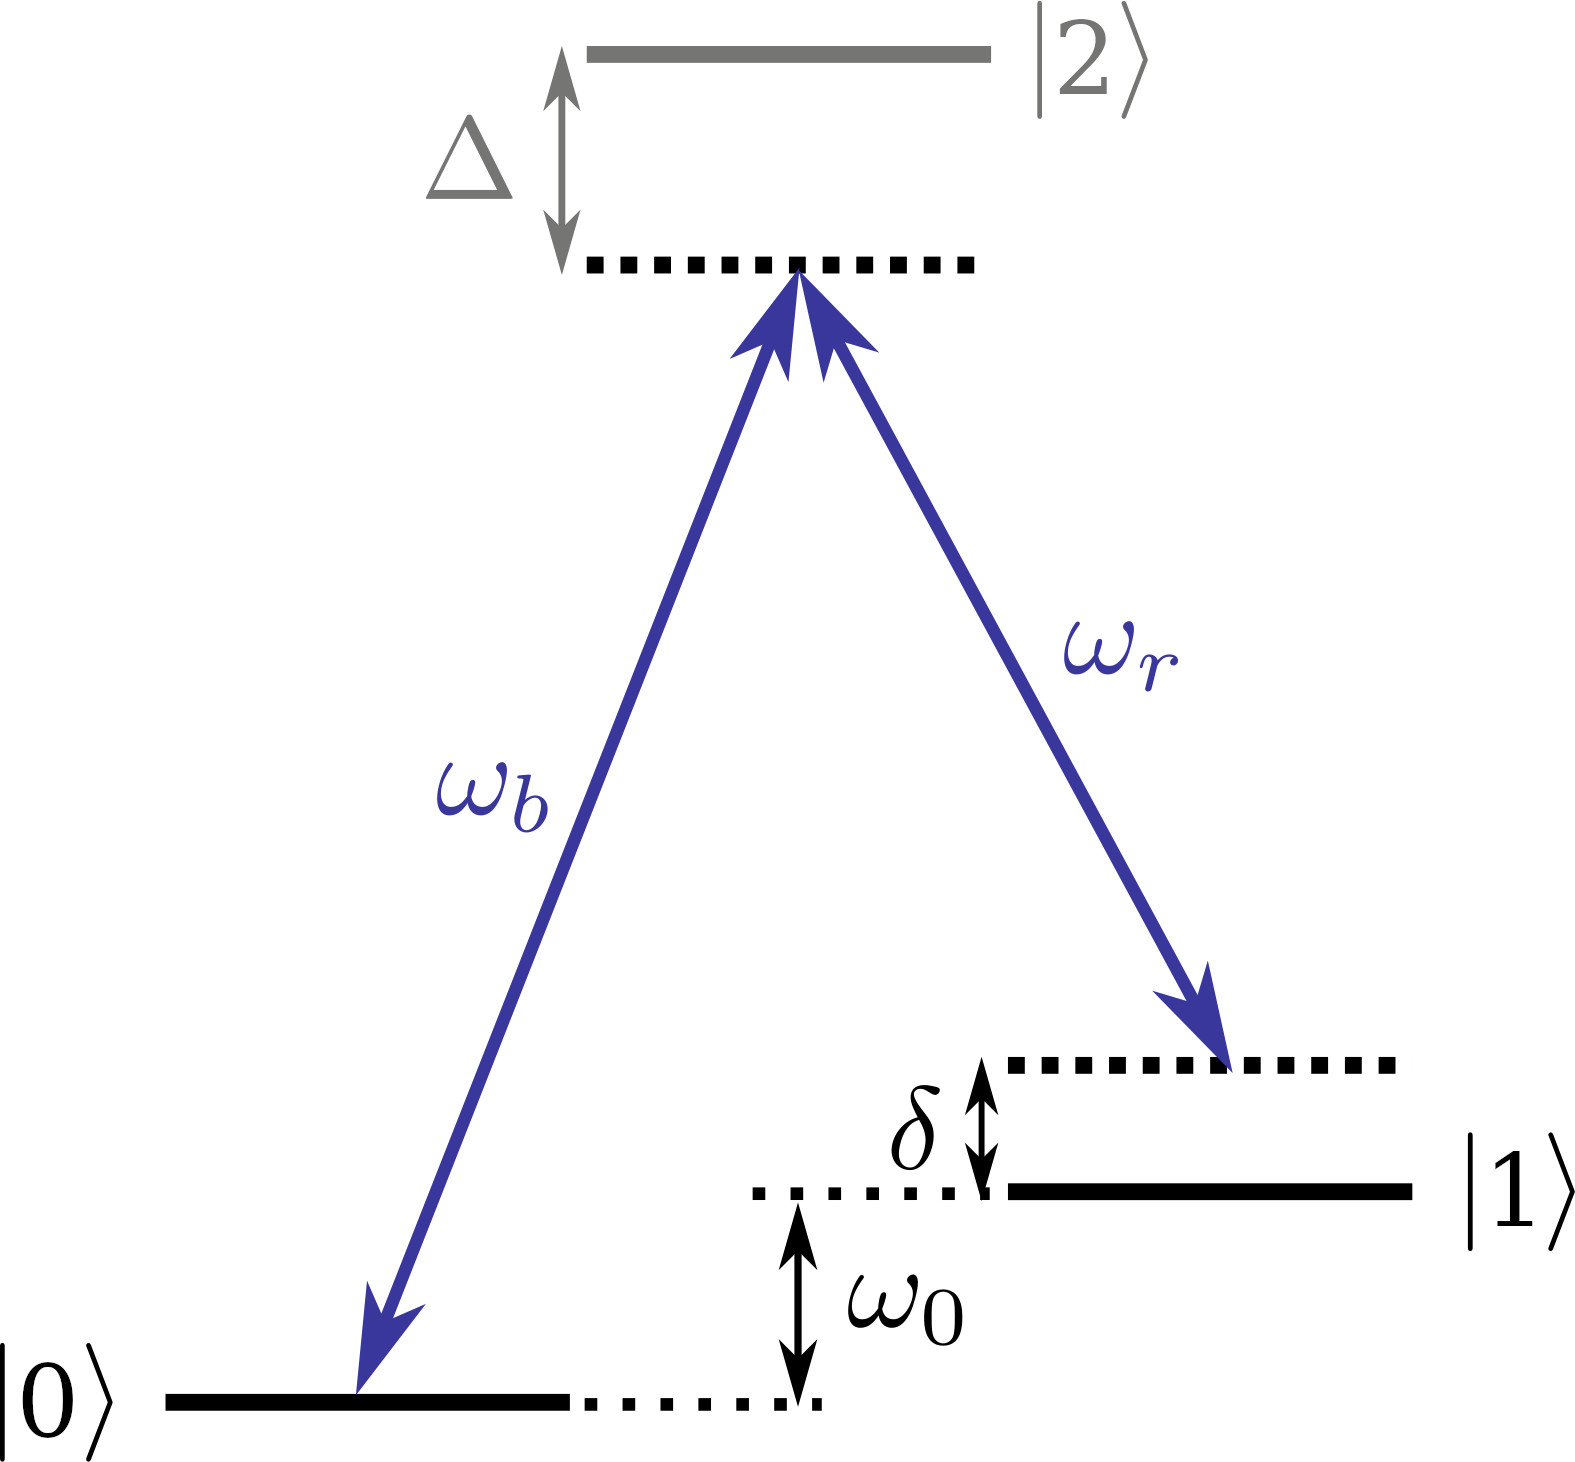
\includegraphics[width=0.3\textwidth]{images/TIQC_raman.jpg}
    \caption{Diagram of the level structure and process of a Raman transition between states \kz and \ko through $\ket{2}$ by use of 2 light beams of energies $\hbar \omega_b > \hbar \omega_r$. Figure taken from \cite{schaferFastGatesMixedSpecies2020}}\label{fig:TIQC_raman}
\end{figure}


\subsection{Single qubit gates}
How specifically single qubit gates are implemented is still highly system dependent, however in all cases it holds true that they only affect the internal state of the given ion.
Here we provide a short summary of which methods are generally used for which qubits.

Optical qubit levels are generally separated by an electric quadrupole transition (or possibly dipole or octupole for shorter and longer excited state lifetimes respectively), thus their gates are very simple and can be implemented by a single light source using the described Rabi oscillations \cite{bruzewiczTrappedionQuantumComputing2019}.
Single qubit gates for hyperfine qubits can be implemented either by a direct transition using microwave radiation or using Raman coupling, which is the most common single gate method for Zeeman qubits as well.
Single gates have been implemented with all of these method with a variety of different qubits and generally their fidelities have been demonstrated to be above 99\%, often better than 99.99\% with gate times usually 5-12 $\si{\micro s}$ \cite{bruzewiczTrappedionQuantumComputing2019}.
Aside from that ultrafast gates have been implemented using $^{171}$Yb$^+$ with times of $50\si{\pico s}$ with fidelities of 99\% \cite{campbellUltrafastGatesSingle2010}.

\subsection{Multi qubit gates}
There is again a variety of methods, we will first describe in detail the CNOT gate theorized by Cirac and Zoller in 1995 \cite{ciracQuantumComputationsCold1995} as it was one of the earliest designs and is often mentioned and cited.
% Here it is necessary to include the effect light has on the collective motional states, however it is a complex process and so is mostly glossed over, more details can be found in for example 

\subsubsection{The Cirac and Zoller CNOT gate \cite{ciracQuantumComputationsCold1995}} This design is specifically for an array of ions confined in a linear Paul trap.
The ions considered as trapped along the 3 dimensions in harmonic potentials at frequencies $f_x, f_y$ and $f_z$ and the ions are (laser) cooled to their ground state.
Their motion can then be described in terms of normal modes and we setup the system so that $f_x, f_y > f_z$ where we take the z axis along the trap, this is so that the modes along the axis are the only to be excited (as it has the lowest energy and also as the excited motional states are well separated).
We also require that the ions internal states has not only the 2 states required for qubits, but another excited internal state that will be used for the operation, notably we only ever use transitions between the ground states and one of the excited states, not between the two excite states directly.

Then as we have an array of N atoms let us use the kets $\ket{0}_n, \ket{1}_n$ and $\ket{2}_n$ to refer to the $n$th atom's internal state and the kets \kz and \ko to refer to the collective motional state.
Then for example $\ket{0}_n\ket{2}_m\ket{1}$ would refer to the state where the $n$th atom is in its ground state, the $m$th atom is in the second excited state and the collective motion is in its excited state, all other atoms can be in any state.

If we then apply an adequately tuned light source to one of the ions so that it couples to one of the internal state transitions and the lowest collective motional state we can achieve entanglement between the two otherwise independent systems.
The theoretical calculation of the tuning can be found in the paper, but in short the laser frequency needs to be detuned by $f_z$ from one of the internal state transitions and the ion position should be at a node of the light wave.
We then use q to denote which of the internal states the light is coupled to, let it be 1 if it couples to the $\ket{0}_n$ to $\ket{1}_n$ transition and 2 for the $\ket{0}_n$ to $\ket{2}_n$ transition ($n$ being whichever ion we illuminate).
We then have the light on for a set amount of time, such that the total phase difference experienced by the ion is $k \pi$, so we can choose $k$ as well.
The effect of this operation can then be described by the following operator

\newcommand{\bigfrac}{(\frac{k\pi}{2})}
\begin{equation}
    \begin{aligned}
        \hat{U}^{k,q}_n &= \ket{0}_n\ket{0}&\bra{0}_n\bra{0} \\
        &+ (\cos{\bigfrac}\ket{0}_n\ket{1} -i e^{i\phi} \sin{\bigfrac}\ket{q}_n\ket{0})&\bra{0}_n\bra{1} \\
        &+ (-i e^{-i\phi} \sin{\bigfrac}\ket{0}_n\ket{1} + \cos{\bigfrac}\ket{q}_n\ket{0})&\bra{q}_n\bra{0} \\
        &+ \ket{q}_n\ket{1}&\bra{q}_n\bra{1}
    \end{aligned}
\end{equation}

which clearly entangles the internal and motional states.
Then to implement a CNOT equivalent gate between 2 ion internal states we will need to apply 3 operations in total, which use the following versions of $\hat{U}^{k,q}_n$.

\begin{equation}
    \begin{aligned}
        \hat{U}^{1,1}_n &= \ket{0}_n\ket{0}&\bra{0}_n\bra{0} \\
        &-i \ket{1}_n\ket{0}&\bra{0}_n\bra{1} \\
        &-i \ket{0}_n\ket{1}&\bra{1}_n\bra{0} \\
        &+ \ket{1}_n\ket{1}&\bra{1}_n\bra{1}
    \end{aligned}
\end{equation}

\begin{equation}
    \begin{aligned}
        \hat{U}^{2,2}_n &= \ket{0}_n\ket{0}&\bra{0}_n\bra{0} \\
        &- \ket{0}_n\ket{1}&\bra{0}_n\bra{1} \\
        &- \ket{2}_n\ket{0}&\bra{2}_n\bra{0} \\
        &+ \ket{2}_n\ket{1}&\bra{2}_n\bra{1}
    \end{aligned}
\end{equation}

The gate is then applied by first cooling the motional state to the ground state so that if we consider the system of some two ions $n$ and $m$ and the total motional state, it will be in a superposition of the following 4 states:
\footnote{Also we only prepare the internal states into $\ket{0}_n$ and $\ket{1}_n$ states all the operations will leave them in these as well so that there is never a $\ket{2}_n$ component at the end of any operation.}
\begin{equation}\label{eqn:ovrl_states}
    \begin{aligned}
        &\ket{0}_n\ket{0}_m\ket{0}, \\
        &\ket{0}_n\ket{1}_m\ket{0}, \\
        &\ket{1}_n\ket{0}_m\ket{0} \text{and} \\
        &\ket{1}_n\ket{1}_m\ket{0}
    \end{aligned}
\end{equation}
and then applying $\hat{U}^{1,1}_n$, $\hat{U}^{2,2}_m$ and $\hat{U}^{1,1}_n$, so that $\hat{G} = \hat{U}^{1,1}_n \hat{U}^{2,2}_m \hat{U}^{1,1}_n$ which will result in the following transformation:
\begin{equation}
    \begin{aligned}
        &\ket{0}_n\ket{0}_m\ket{0} \rightarrow & \ket{0}_n\ket{0}_m\ket{0} \rightarrow & \ket{0}_n\ket{0}_m\ket{0} \rightarrow & \ket{0}_n\ket{0}_m\ket{0} \\
        &\ket{0}_n\ket{1}_m\ket{0} \rightarrow & \ket{0}_n\ket{1}_m\ket{0} \rightarrow & \ket{0}_n\ket{1}_m\ket{0} \rightarrow & \ket{0}_n\ket{1}_m\ket{0} \\
        &\ket{1}_n\ket{0}_m\ket{0} \rightarrow & -i\ket{0}_n\ket{0}_m\ket{1} \rightarrow & +i\ket{0}_n\ket{0}_m\ket{1} \rightarrow & \ket{1}_n\ket{0}_m\ket{0} \\
        &\ket{1}_n\ket{1}_m\ket{0} \rightarrow & -i\ket{0}_n\ket{1}_m\ket{1} \rightarrow & -i\ket{0}_n\ket{1}_m\ket{1} \rightarrow & -\ket{1}_n\ket{1}_m\ket{0}
    \end{aligned}
\end{equation}

To see how this is equivalent to a CNOT consider expressing the $m$th ion's state in the basis $\ket{\pm}_m = \frac{\ket{0}_m \pm \ket{1}_m}{\sqrt{2}}$.
It might be clear that in this basis $\hat{G}$ is the CNOT gate, if not then note that the Hadamard gate represents the transformation between the $\ket{0/1}_m$ and $\ket{\pm}_m$ basis, meaning we can apply the single qubit Hadamard to qubit $m$ before and after applying $\hat{G}$ to get a typical CNOT, in matrix representation where we take the states in the same order as in \cref{eqn:ovrl_states} it is done as follows
\begin{equation}
    \hat{H_m}\hat{G}\hat{H_m} \leftrightarrow \frac{1}{2}
    \begin{pmatrix}
        1 & 0 & 0 & 0 \\
        0 & 1 & 0 & 0 \\
        0 & 0 & 1 & 1 \\
        0 & 0 & 1 & -1
    \end{pmatrix}
    \begin{pmatrix}
        1 & 0 & 0 & 0 \\
        0 & 1 & 0 & 0 \\
        0 & 0 & 1 & 0 \\
        0 & 0 & 0 & -1
    \end{pmatrix}
    \begin{pmatrix}
        1 & 0 & 0 & 0 \\
        0 & 1 & 0 & 0 \\
        0 & 0 & 1 & 1 \\
        0 & 0 & 1 & -1
    \end{pmatrix} = 
    \begin{pmatrix}
        1 & 0 & 0 & 0 \\
        0 & 1 & 0 & 0 \\
        0 & 0 & 0 & 1 \\
        0 & 0 & 1 & 0
    \end{pmatrix}
\end{equation}

Which is a recognisable CNOT, the Cirac and Zoller gate is one of the first to be theorized and demonstrated \cite{monroeDemonstrationFundamentalQuantum1995}, both in 1995, since then it has often been cited.
Though many other designs have been developed they generally rely on similar techniques, specifically on coupling the ions internal states through their motion, it is often described as a quantum bus.





% \section{State Prep and Readout}
% Mention -- https://jonathan-hui.medium.com/qc-how-to-build-a-quantum-computer-with-trapped-ions-88b958b81484 -- as primary source?
% Maybe need to mention cooling, seems to be primary step in creating stable |0> and |1> states ; need optical pumping, raman cooling, etc. ; once cooled to stable motional ground state, then can be excited with laser of appropriate frequency to |1>, which causes atom to fluoresce for readout
% Optical pumping is well-known well-working technique, so DVC2 is easily satisfied because easy to initialise qubits in ground state this way
% |0> and |1> will have different energies, so by using light of specific frequency that can only excite for e.g. |0> to some auxiliary level, then if the electron is in |0> it will excite and return back to original state by emitting light again so if we see a glow when we shine light of this frequency that means electron was in |0> after the calculation but otherwise if it stays dark it means electron was in |1> because the light we shone did not excite anything in the ground state because there was nothing there to excite


